\documentclass[article]{elsarticle}
\usepackage{amsmath}
\usepackage{lineno,hyperref}
\usepackage{graphicx}
\graphicspath{ {./images/} }

\modulolinenumbers[5]

\journal{Journal of Insignificant Results}

\bibliographystyle{elsarticle-num}
%%%%%%%%%%%%%%%%%%%%%%%

\begin{document}

\begin{frontmatter}

\title{Resumen del tema 3 - Introducción al método científico en investigación}

\author{Manuel Pasieka\corref{fn_autor1}}
\cortext[fn_autor1]{Corresponding author}
\ead{manuel.pasieka@protonmail.ch}

\begin{abstract}
En este trabajo darnos una introducción a los aspectos básicos del método científico, al tema de la publicación científica y al sistema Látex. 
\end{abstract}

\begin{keyword}
método científico \sep publicación scientifica \sep \LaTeX
\end{keyword}

\end{frontmatter}

%%\linenumbers

\section{Introducción}
El tema 3 de la asignatura Investigación en Inteligencia Artificial explica los siguientes puntos

\begin{itemize}
\item El método científico
\item Fuentes y maneras de buscar literatura científica
\item El proceso de la publicación de un artículo científico
\item Aspectos éticos relacionados con el tema de plagia ismo académico
\item Herramientas útiles para organizar documentos (i.e mendelay)
\item Látex para escribir textos científicos
\end{itemize}

\vspace{1.5\baselineskip}

Este resumen va a ocuparse con solo algunos de estos temas.

\section{El método científico}

El método científico sirve para entender mejor el mundo y nuestra posición en ello.
Es un sistema de investigación desarrollado desde el siglo diez y seis por
investigadores como Galileo Galilei, René Descartes o Francis Bacon.

\vspace{1.5\baselineskip}

Tiene tres pilares y conceptos que definen el método científico

\begin{itemize}
\item \textbf{Lo empírico}: La base de cada objeto estudiado por la ciencia
    tiene que ser un hecho en el mundo real
\item \textbf{La medición}: Para ser real vale algo que es mensurable
\item \textbf{Razonamiento}: Para algo ser cierto o entendido, tiene que ser
    hecho, mensurable y hay que existir una razón y una explicación por su existencia.
\end{itemize}

\vspace{1.5\baselineskip}

Además, tiene en común todos los conocimientos logrados por el método científico:
\begin{itemize}
\item \textbf{La reproducibilidad}: las tres características (empírico,
    mensurable, razonable) tiene que ser repetible para cualquier investigador,
    donde o cuando sea
\item \textbf{La refutabilidad}: un conocimiento nunca puede ser verificado,
    sin dudas, solo quedarse no corregido por otra hipótesis que de una o otra
    manera explica mejor las mediciones o razonamientos al aspecto del tema.
\end{itemize}

\vspace{1.5\baselineskip}

El método científico en muchas ocasiones es descrito como un proceso continúe de los pasos
explicados en la figura \ref{fig1}.

\begin{figure}[h]
\centering
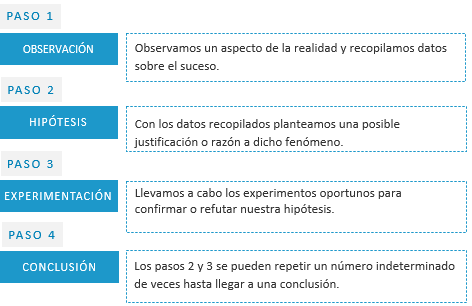
\includegraphics[width=0.5\textwidth]{img1}
\caption{Pasos tipícos del metodo scientifico}
\label{fig1}
\end{figure}

\vspace{1.5\baselineskip}

En general el orden de estos pasos no es fijo y una vez llegado a una conclusión,
se hacen nuevas hipótesis que, para estudiarles, necesitan nueves observaciones.

\newpage
\section{La publicación de artículos científicos}

El avance científico depende de la comunicación y el intercambio de descubrimientos entre científicos. \par

La manera tradicional de comunicar sus propios descubrimientos al mundo, son las
revistas científicas que ayudan en distribuir estos descubrimientos, filtran los
diferentes trabajos por temas y relevancia y ayudan de verificar la calidad del
trabajo en el caso de una revista que utiliza ‘peer review’.

Aunque en los días de hoy con el internet, donde el intercambio de información
es muy fácil y aún libre, las revistas siguen tener una gran importancia en el
mundo científico.

\vspace{1.5\baselineskip}

Eso mas que todo es porque se utiliza como métrica de evaluar la cualidad del
trabajo de un científico. Cada revista tiene un valor der cualidad basando en el
numero de citas de sus artículos (por ejemplo, el Journal Citation Report) y si
un científico consigue publicar su trabajo en revistas de alta cualidad se asume
que este científico es bueno y su trabajo es importante.

\vspace{1.5\baselineskip}

Este sistema tiene como aventaje que alguien fuera del campo científico puede
evaluar el científico, sin entender su trabajo, pero también dirige la manera
como los científicos hacen sus investigaciones. Eso significa en concreto que
la mayoría de los científicos solo puede permitirse estudiar temas populares;
algo que llamar la atención a la comunidad científica, y al otro lado les obliga
a descubrir y a adaptar sus trabajos y resultados para que sean significante,
sorprendente y más que todo, nuevo.

\vspace{1.5\baselineskip}

La situación se pone peor aun, porque las revistas, aunque piden miles de euros
a los autores por publicación, también piden el lector que page por su acceso.

En particular este acceso restringido a las novedades de la ciencia acumuló en
un movimiento llamado ‘open access’ que quiere conseguir un acceso libre y
gratuita a las publicaciones científicas.

Para conseguir eso hay diferentes iniciativas.
\begin{itemize}
\item \textbf{Sci-hub.tw} : es una comunidad que ofrece gratuita artículos robados de diferentes revistas
\item \textbf{Arxvid.org y bioRxiv.org} : plataformas para publicar artículos gratis y con acceso libre 
\end{itemize}

Estos iniciativas de ‘open access’ tienen un efecto relevante y positivo para
la comunidad científica, mas que todo para científicos en regiones menos
desarrollados \cite{Evans2009}. \par

\newpage
\section{Ejemplos de Látex}
El siguiente son algunos ejemplos simples de que es posible con el sistema Látex
al aspecto de formar y gestión textos científicos.

\vspace{1.5\baselineskip}

\begin{tabular}{l|c|c}
    Tipo de Ejemplo   & Ejemplo A & Ejemplo B  \\
    \hline
    \hline
    Formulas &\(k_{n+1} = n^2 + k_n^2 - k_{n-1}\)   & \( f(n) = n^5 + 4n^2 + 2 |_{n=17} \) \\
    Formulas & \( \frac{n!}{k!(n-k)!} = \binom{n}{k} \) & \( \sqrt[n]{1+x+x^2+x^3+\dots+x^n} \) \\
    Referencias & Tech Report 1\cite{Hughes2007} & The Brain in a vat \cite{Putnam1994} \\
    Referencias & One Billion Dollars for a Conscious Robot \cite{Bringsjord2007} & What Is It Like to Be A Bat? \cite{Nagel1974}\\
\end{tabular}

\vspace{1.5\baselineskip}

\section{Resumen}
Este trabajo corto intentó de da una introducción al tema del método científico,
a la situación actual y algunos aspectos de la publicación científica, y a técnicos de látex.

\section*{References}

\bibliography{bibfile}

\end{document}